%\documentclass{beamer} %voce pode usar este modelo tambem
\documentclass[t,handout,9pt]{beamer}
\usepackage{graphicx}
\usepackage{url}
\usepackage[british]{babel}
%\batchmode
% \pgfpagesuselayout{4 on 1}[letterpaper,landscape,border shrink=5mm]
\usepackage{amsmath}
\usepackage{amssymb}
\usepackage{amsfonts}
\usepackage{enumerate}
\usepackage{epsfig}
\usepackage{bbm}
\usepackage{calc}
\usepackage{adjustbox}
\usepackage{color}
\usepackage{ifthen}
\usepackage{capt-of}
\usepackage{float}
\usepackage{booktabs}
\usepackage{dcolumn}
\usepackage{multicol}
\usepackage{hyperref}
\usepackage[flushleft]{threeparttable}
\usepackage{subcaption}
\usepackage{adjustbox}
\usepackage{ragged2e}
\usepackage{xcolor}
\usepackage{pgfpages}
%\usepackage{showframe}

\usepackage{cmbright}

\renewcommand\ttdefault{cmvtt} % selects CM typewriter

\usepackage[utf8]{inputenc} % Required for inputting international characters
\usepackage[T1]{fontenc} 	% Output font encoding for international characters

%\DeclareFontShape{OT1}{cmss}{b}{n}{<->ssub * cmss/bx/n}{}

\usetheme[compress]{Berlin}
\definecolor{sapienza}{RGB}{0, 49, 83}
\usecolortheme[named=sapienza]{structure}

\usepackage[backend=bibtex,style=alphabetic,giveninits=true,url=false,eprint=false,doi=false]{biblatex}
\DeclareNameAlias{sortname}{last-first}
\renewcommand*{\nameyeardelim}{\addcomma\addspace}
\renewcommand*{\bibfont}{\footnotesize}
\addbibresource{example.bib}
\setbeamerfont{footnote}{size=\tiny}

\setbeamerfont{title}{size=\LARGE}

% reduce spaces between tables/figures and caption
\usepackage[font=small,skip=1pt]{caption}

%% pgf plots stuff
%\usepackage{pgfplots}
%\pgfplotsset{compat=newest}
%% the following commands are needed for some matlab2tikz features
%\usetikzlibrary{plotmarks}
%\usetikzlibrary{arrows.meta}
%\usepgfplotslibrary{patchplots}

% one navigation dot per slide trick
\AtBeginSection[]{\subsection{}}

% fix misbehave for allowframebreaks
\usepackage{etoolbox}
\makeatletter
\patchcmd{\slideentry}{\ifnum#2>0}{\ifnum2>0}{}% replace the subsection number test with a test that always returns true
% use frame numbers instead of subsection slide numbers so that frames broken over slides get separate circles
\patchcmd{\slideentry}{\c@subsectionslide}{\c@framenumber}{}{\@error{unable to patch}}
\patchcmd{\beamer@writeslidentry}{\c@subsectionslide}{\c@framenumber}{}{\@error{unable to patch}}

% date in footer trick
\makeatletter
  \setbeamertemplate{footline}{%
    \begin{beamercolorbox}[colsep=1.5pt]{upper separation line foot}
    \end{beamercolorbox}
    \begin{beamercolorbox}[ht=2.5ex,dp=1.125ex,%
      leftskip=.3cm,rightskip=.3cm plus1fil]{author in head/foot}%
      \leavevmode{\usebeamerfont{author in head/foot}\insertshortauthor}%
      \hfill%
      {\usebeamerfont{institute in head/foot}\usebeamercolor[fg]{institute in head/foot}\insertshortinstitute}%
    \end{beamercolorbox}%
    \begin{beamercolorbox}[ht=2.5ex,dp=1.125ex,%
      leftskip=.3cm,rightskip=.3cm plus1fil]{title in head/foot}%
      {\usebeamerfont{title in head/foot}\insertshorttitle\hfill\insertshortdate}%
    \end{beamercolorbox}%
    \begin{beamercolorbox}[colsep=1.5pt]{lower separation line foot}
    \end{beamercolorbox}
  }
\makeatletter

% remove dot for titlepage and Outline
\makeatletter
\let\old@beamer@writeslidentry\beamer@writeslidentry
\def\beamer@writeslidentry{%
  \expandafter\beamer@ifempty\expandafter{\beamer@framestartpage}{}% does not happen normally
  {%else
    \clearpage\beamer@notesactions%
  }
}
\makeatother

% let's number figure captions
\setbeamertemplate{caption}[numbered]

% trick for grouping equations
\newenvironment{rcases}
  {\left.\begin{aligned}}
  {\end{aligned}\right\rbrace}

%-------------------------Titulo/Autores/Orientador------------------------------------------------
\title[Introduction to Computer Programming]{Introduction to Computer Programming}
\date[A.Y. 2024-2025]{\\A.Y. 2024-2025}
\author[Alessio Martino]{Prof. Alessio Martino\\
\smallskip
{\small \href{mailto:amartino@luiss.it}{\texttt{amartino@luiss.it}}}\\
\smallskip
}
\institute[24/09/2024]{Department of Business and Management\\Viale Romania 32, 00197 Rome\\[\bigskipamount]

\includegraphics[scale=0.4]{Figures/cliente-luiss.png}%
}

%-------------------------Logo na parte de baixo do slide------------------------------------------
%\pgfdeclareimage[height=0.7cm]{senac-logo}{senac-logo.pdf}
%\logo{\pgfuseimage{senac-logo}\hspace*{0.5cm}}

%-------------------------Este código faz o menuzinho bacana na parte superior do slide------------
%\AtBeginSection[]
%{
%  \begin{frame}<beamer>
%    \frametitle{Outline}
%    \tableofcontents[currentsection]
%  \end{frame}
%}
%\beamerdefaultoverlayspecification{<+->}
% -----------------------------------------------------------------------------

\begin{document}
% -----------------------------------------------------------------------------

%---Gerador de Sumário---------------------------------------------------------

\frame[noframenumbering]{
	\titlepage
}

% begin personalization stuff
\setbeamertemplate{navigation symbols}{%
	\insertslidenavigationsymbol
	\insertframenavigationsymbol
	\insertsubsectionnavigationsymbol
	\insertsectionnavigationsymbol
	\insertdocnavigationsymbol
	\insertbackfindforwardnavigationsymbol
	\hspace{1em}%
	\usebeamerfont{footline}
	\insertframenumber/\inserttotalframenumber%
}
\setbeamertemplate{itemize items}[circle]
\setbeamertemplate{enumerate items}[circle]
\setbeamertemplate{bibliography item}{\insertbiblabel}
% end personalization stuff

\section[]{}
\begin{frame}{Outline}
	\tableofcontents
\end{frame}
%\begin{frame}{Outline}
%\begin{multicols}{2}
%  \tableofcontents
%\end{multicols}
%\end{frame}
%---Fim do Sumário------------------------------------------------------------

% reset navigation dots for other slides
\makeatletter
\let\beamer@writeslidentry\old@beamer@writeslidentry
\makeatother

% -----------------------------------------------------------------------------
\section{Branching}
\begin{frame}{Branching}
\adjustbox{valign=t}{\begin{minipage}[t]{0.49\textwidth}
%\vspace{0.3cm}
A program \textcolor{red}{without branching}\\

\includegraphics[height=0.8\textheight]{Figures/Branching1}
\end{minipage}}%
\hfill
\adjustbox{valign=t}{\begin{minipage}[t]{0.49\textwidth}
%\vspace{0.3cm}
A program \textcolor{red}{with branching}\\

\includegraphics[height=0.8\textheight]{Figures/Branching2}
\end{minipage}}
\end{frame}
%
\subsection{Branching in Python}
\begin{frame}
\adjustbox{valign=t}{\begin{minipage}[t]{0.3\textwidth}
%\vspace{0.3cm}
Plain \texttt{if}\\
\begin{table}[]
\begin{flushleft}
\begin{tabular}{ll}
\texttt{if <condition>:} &  \\
\texttt{\qquad statement}        & \\
\texttt{\qquad statement}        & \\
\texttt{\qquad statement}        & \\
\texttt{\qquad statement}        & \\
\end{tabular}
\end{flushleft}
\end{table}
\end{minipage}}%
\hfill
\adjustbox{valign=t}{\begin{minipage}[t]{0.3\textwidth}
\texttt{if}--\texttt{else}\\
%\vspace{-0.4cm}
\begin{table}[]
\begin{flushleft}
\begin{tabular}{ll}
\texttt{if <condition>:} &  \\
\texttt{\qquad statement}        & \\
\texttt{\qquad ...}        & \\
\texttt{\qquad statement}        & \\
\texttt{else:} &  \\
\texttt{\qquad statement}        & \\
\texttt{\qquad ...}        & \\
\texttt{\qquad statement}        & \\
\end{tabular}
\end{flushleft}
\end{table}
\end{minipage}}%
\hfill
\adjustbox{valign=t}{\begin{minipage}[t]{0.3\textwidth}
\texttt{if}--\texttt{else if}--\texttt{else}\\
\vspace{-0.4cm}
\begin{table}[]
\begin{flushleft}
\begin{tabular}{ll}
\texttt{if <condition>:} &  \\
\texttt{\qquad statement}        & \\
\texttt{\qquad ...}        & \\
\texttt{\qquad statement}        & \\
\texttt{elif <condition>:} &  \\
\texttt{\qquad statement}        & \\
\texttt{\qquad ...}        & \\
\texttt{\qquad statement}        & \\
\texttt{else:} &  \\
\texttt{\qquad statement}        & \\
\texttt{\qquad ...}        & \\
\texttt{\qquad statement}        & \\
\end{tabular}
\end{flushleft}
\end{table}
\end{minipage}}
\begin{itemize}
	\item \texttt{<condition>} yields \texttt{True} or \texttt{False}
	\item evaluate statements in that block if \texttt{<condition>} is \texttt{True}
	\item indentation is the key to delimit blocks
	\item place \texttt{:} at the end of \texttt{<condition>}
\end{itemize}
\end{frame}
%
\section{Examples}
\begin{frame}{Examples}
\vfill
Examples \texttt{if}.\\
\vfill
\begin{table}[]
\begin{flushleft}
\begin{tabular}{ll}
\texttt{num = 3} &  \\
\texttt{if num>0:} &  \\
\texttt{\qquad print(num, "is a positive number.")}        & \\
\texttt{print("This is always printed. It's outside of the block.")} &  \\
\end{tabular}
\end{flushleft}
\end{table}
\vfill
\begin{table}[]
\begin{flushleft}
\begin{tabular}{ll}
\texttt{num = -1} &  \\
\texttt{if num>0:} &  \\
\texttt{\qquad print(num, "is a positive number.")}        & \\
\texttt{print("This is always printed. It's outside of the block.")} &  \\
\end{tabular}
\end{flushleft}
\end{table}
\vfill
\end{frame}
%
\begin{frame}
\vfill
\begin{figure}
\centering
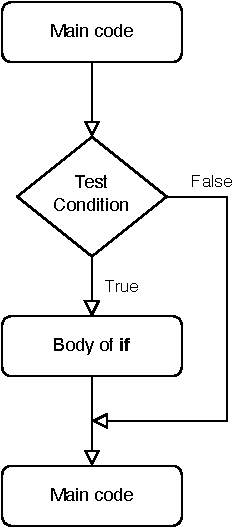
\includegraphics[height=0.8\textheight]{Figures/branching-if}
\caption{Logical flowchart of an \texttt{if} statement.}
\end{figure}
\vfill
\end{frame}
%
\begin{frame}
\vfill
Examples \texttt{if}--\texttt{else}.\\
\vfill
\begin{table}[]
\begin{flushleft}
\begin{tabular}{ll}
\texttt{num = 1} &  \\
\texttt{if num>=0:} &  \\
\texttt{\qquad print("Number is positive or zero.")}        & \\
\texttt{else:} &  \\
\texttt{\qquad print("Negative number.")} &  \\
\end{tabular}
\end{flushleft}
\end{table}
\vfill
What happens with
\begin{itemize}
	\item \texttt{num=0}
\end{itemize}
or
\begin{itemize}
	\item \texttt{num=-5}
\end{itemize}
\vfill
\end{frame}
%
\begin{frame}
\vfill
\begin{figure}
\centering
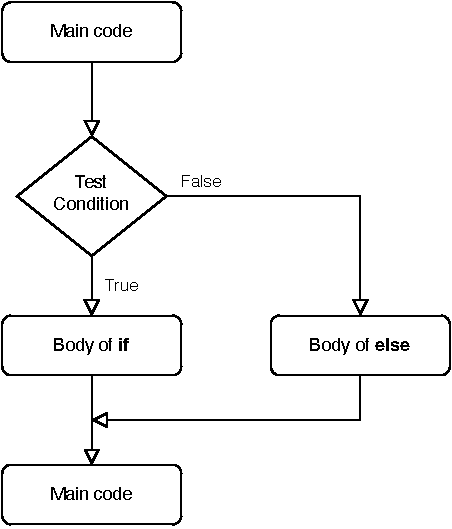
\includegraphics[height=0.8\textheight]{Figures/branching-if-else}
\caption{Logical flowchart of an \texttt{if-else} statement.}
\end{figure}
\vfill
\end{frame}
%
\begin{frame}
\vfill
Examples \texttt{if}--\texttt{elif}--\texttt{else}.\\
\vfill
\begin{table}[]
\begin{flushleft}
\begin{tabular}{ll}
\texttt{num = 3.4} &  \\
\texttt{if num>0:} &  \\
\texttt{\qquad print("Number is positive.")}        & \\
\texttt{elif num==0:} &  \\
\texttt{\qquad print("Number is zero.")} &  \\
\texttt{else:} &  \\
\texttt{\qquad print("Number is negative.")} &  \\
\end{tabular}
\end{flushleft}
\end{table}
\vfill
What happens with
\begin{itemize}
	\item \texttt{num=0}
\end{itemize}
or
\begin{itemize}
	\item \texttt{num=-4.5}
\end{itemize}
\vfill
\end{frame}
%
\begin{frame}
\vfill
\begin{figure}
\centering
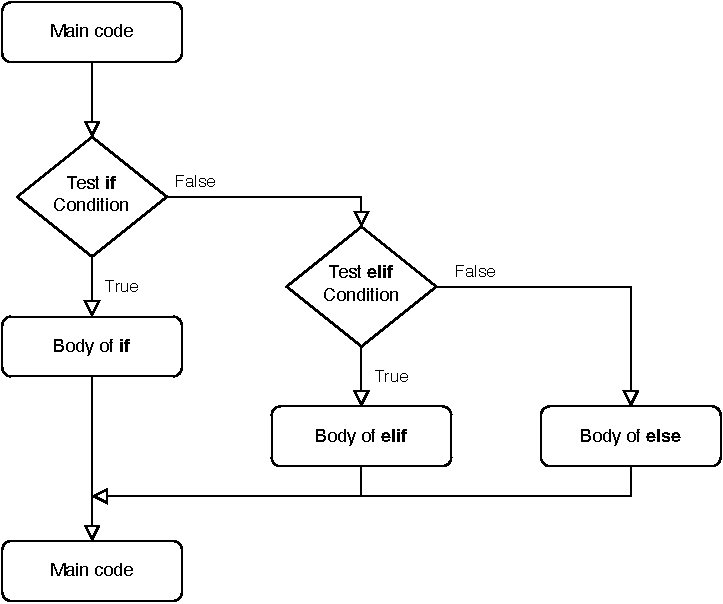
\includegraphics[height=0.8\textheight]{Figures/branching-if-elif-else}
\caption{Logical flowchart of an \texttt{if-elif-else} statement.}
\end{figure}
\vfill
\end{frame}
%
\section{Nested Statements}
\begin{frame}{Nested Statements}
Branching statements \texttt{if}, \texttt{else} and \texttt{elif} can be nested arbitrarily.
\begin{table}[]
\begin{flushleft}
\begin{tabular}{ll}
\texttt{num = input("Enter a number: ")} & \\
\texttt{num = float(num)} & $\leftarrow$ recall: \texttt{"input()"} yields a string\\
\texttt{if num>=0:} & \\
\texttt{\qquad if num==0:} & \\
\texttt{\qquad\qquad print("Number is zero")} & \\
\texttt{\qquad else:} & \\
\texttt{\qquad\qquad print("Number is positive")} & \\
\texttt{else:} & \\
\texttt{\qquad print("Number is negative")} & \\
\end{tabular}
\end{flushleft}
\end{table}
\end{frame}
%
\section{Indentation}
\begin{frame}{Indentation}
\begin{block}{Recall}
Indentation (tab or 4 spaces) delimits blocks of code in Python.
\end{block}
\begin{table}[]
\begin{flushleft}
\begin{tabular}{ll}
\texttt{x = float(input("Enter a value for x: "))} & \\
\texttt{y = float(input("Enter a value for y: "))} & \\
\texttt{if x==y:} & \\
\colorbox{pink}{\texttt{\qquad print("y and x are equal")}} & \\
\colorbox{pink}{\texttt{\qquad if y!=0:}} & \\
\colorbox{magenta}{\texttt{\qquad\qquad print("Finally, x/y is", x/y)}} & \\
\texttt{elif x>y:} & \\
\colorbox{pink}{\texttt{\qquad print("y is smaller")}} & \\
\texttt{else:} & \\
\colorbox{pink}{\texttt{\qquad print("x is smaller")}} & \\
\end{tabular}
\end{flushleft}
\end{table}
\end{frame}
%------------------------------------------------------------------------------
\section{Exercises}
\begin{frame}{Exercises}
\vfill
\begin{enumerate}
	\item Write a piece of code that checks whether a number is even.\\If so, print a message.
\end{enumerate}
\vfill
A possible solution follows:
\begin{table}[]
	\begin{tabular}{ll}
	\texttt{num = 42} & \\
	\texttt{if num \% 2 == 0:} & \\
	\texttt{\qquad print("Condition evaluates to True.")} & \\
	\texttt{\qquad print("Number", num, "is even")} & \\
	\end{tabular}
	\end{table}
\vfill
\end{frame}
%
\begin{frame}
\vfill
\begin{enumerate}
\setcounter{enumi}{1}
	\item Write a piece of code that checks whether a number is even. Print a message about the outcome (odd or even).
\end{enumerate}
\vfill
A possible solution follows:
\begin{table}[]
	\begin{tabular}{ll}
	\texttt{num = 42} & \\
	\texttt{if num \% 2 == 0:} & \\
	\texttt{\qquad print("Condition evaluates to True.")} & \\
	\texttt{\qquad print("Number", num, "is even")} & \\
	\texttt{else:} & \\
	\texttt{\qquad print("Condition evaluates to False.")} & \\
	\texttt{\qquad print("Number", num, "is odd")} & \\
	\end{tabular}
	\end{table}
\vfill
\end{frame}
%
\begin{frame}
\vfill
\begin{enumerate}
\setcounter{enumi}{2}
	\item Write a piece of code that checks whether a number is odd or even. Assign a proper value (e.g., 'odd' or 'even') to a variable, depending on the outcome of the condition. Print the outcome at the end.
\end{enumerate}
\vfill
A possible solution follows:
\begin{table}[]
	\begin{tabular}{ll}
	\texttt{num = 42} & \\
	\texttt{if num \% 2 == 0:} & \\
	\texttt{\qquad parity = "even"} & \\
	\texttt{else:} & \\
	\texttt{\qquad parity = "odd"} & \\
	\texttt{print("Number", num, "is", parity)} & \\
	\end{tabular}
	\end{table}
\vfill
\end{frame}
%
\begin{frame}
\vfill
\begin{enumerate}
\setcounter{enumi}{3}
	\item Write a piece of code that checks whether a number is divisible by 2, 3, 5 and 7.
\end{enumerate}
\vfill
A possible solution follows:
\begin{table}[]
	\begin{tabular}{ll}
	\texttt{num = 42} & \\
	\texttt{if num \% 2 == 0:} & \\
	\texttt{\qquad print("Number ", num, "is divisible by 2.")} & \\
	\texttt{if num \% 3 == 0:} & \\
	\texttt{\qquad print("Number ", num, "is divisible by 3.")} & \\
	\texttt{if num \% 5 == 0:} & \\
	\texttt{\qquad print("Number ", num, "is divisible by 5.")} & \\
	\texttt{if num \% 7 == 0:} & \\
	\texttt{\qquad print("Number ", num, "is divisible by 7.")} & \\
	\end{tabular}
	\end{table}
\vfill
\end{frame}
%
\begin{frame}
\vfill
\begin{enumerate}
\setcounter{enumi}{4}
	\item Write a piece of code that checks whether a number is odd or even. Print a message informing the user.\\If odd, check whether the number is divisible by 5. Print a message informing the user. If even, check whether the number is divisible by 3. Print a message informing the user.
\end{enumerate}
A possible solution follows:
\begin{table}[]
	\begin{tabular}{ll}
	\texttt{num = 15} & \\
	\texttt{if num \% 2 == 0:} & \\
	\texttt{\qquad print("Number", num, "is even.")} & \\
	\texttt{\qquad if num \% 3 == 0:} & \\
	\texttt{\qquad\qquad print("Number", num, "is also divisible by 3.")} & \\
	\texttt{\qquad else:} & \\
	\texttt{\qquad\qquad print("Number", num, "is not divisible by 3.")} & \\
	\texttt{else:} & \\
	\texttt{\qquad print("Number", num, "is odd.")} & \\
	\texttt{\qquad if num \% 5 == 0:} & \\
	\texttt{\qquad\qquad print("Number", num, "is also divisible by 5.")} & \\
	\texttt{\qquad else:} & \\
	\texttt{\qquad\qquad print("Number", num, "is not divisible by 5.")} & \\
	\end{tabular}
	\end{table}
\vfill
\end{frame}
%
\begin{frame}
\vfill
\begin{enumerate}
\setcounter{enumi}{5}
	\item Write a piece of code that asks the user to insert the dog's age in human's years and calculates a dog's age in dog's years.\\For the first two years, a dog year is equal to 10.5 human years. After that, each dog year equals 4 human years.
\end{enumerate}
A possible solution follows:
\begin{table}[]
	\begin{tabular}{ll}
	\texttt{h\_age = int(input("Input a dog's age in human years: "))} & \\
	\texttt{if h\_age <= 0:} & \\
	\texttt{\qquad print("Age must be a positive number.")} & \\
	\texttt{else:} & \\
	\texttt{\qquad if h\_age <= 2:} & \\
	\texttt{\qquad\qquad d\_age = h\_age * 10.5} & \\
	\texttt{\qquad else:} & \\
	\texttt{\qquad\qquad d\_age = 10.5 + 10.5 + (h\_age - 2) * 4} & \\
	\texttt{\qquad print("The dog's age in dog's years is:", d\_age)} & \\
	\end{tabular}
	\end{table}
\vfill
\end{frame}
%------------------------------------------------------------------------------
%\section{References}
%\begin{frame}[allowframebreaks]{References}
%%\bibliographystyle{apacite}
%\printbibliography[heading=none]
%\end{frame}
\section{References}
\begin{frame}{References}
\begin{itemize}
	\item Guttag, J. V. (2013). \textit{Introduction to Computation and Programming using Python (Revised and Expanded Edition)}. MIT Press. [Chapter 2]
	\item Downey, A. (2015). \textit{Think Python}. Green Tea Press ed. 2nd. [Sections 5.4--5.7]
\end{itemize}
\end{frame}
%------------------------------------------------------------------------------
\section{Acknowledgments}
\begin{frame}{Acknowledgments}
% \begin{itemize}
% 	\item Prof. Irene Finocchi (LUISS University)\\
% 	\quad \textit{Introduction to Computer Programming} Lecture Notes (2020-2021)
% \end{itemize}
\end{frame}
%------------------------------------------------------------------------------
%\subsection{Sites legais}
%\begin{frame}{Sites legais}
%  Want to know more? See!
%  \begin{itemize}
%    \item Browse in my page \url{http://www.ezefranca.com}.
%    \item Browse on BCC page \url{http://www.sp.senac.br/bcc}.
%    \item Thanks WriteLaTeX from Support! \url{http://www.writelatex.com}.
%  \end{itemize}
%
%\end{frame}
%------------------------------------------------------------------------------

% -----------------------------------------------------------------------------
\end{document}
%-----------------------------------------------Este comentario nunca aparecera
